  %%%%%%%%%%%%%%%%%%%%%%%%%%%%%%%%%%%%%%% -*- coding: utf-8; mode: latex -*- %%
  %
%%%%%                         CHAPTER RELATED WORK
%
%

  %%%%%%%%%%%%%%%%%%%%%%%%%%%%%%%%%%%%%%%%%%%%%%%%%%%%%%%%%%%%%%%%%%%%%%%%%%%%%
  %
%%%%%                     HEAD MATTER
 %%%
  %
 

\chapter{Related Work}

\label{ch:relatedwork}

\begin{quotation}
No sensible decision can be made any longer without taking into account not only the world as it is, but the world as it will be.
{\small\it -- Isaac Asimov, writer and scientist (1919 - 1992)}
\end{quotation}

The database market is currently divided in three major segments. DataWarehouses (used for business intelligence), OLTP systems and lastly another set of systems which are currently the most innovative and fast-evolving in that market. In this thesis work, the focus is therefore on the third type, so called NoSQL systems for instance.

NoSQL databases are the evolution of traditional RDBMSs, they are the current underlying technology that powers many of the distributed applications we find nowadays on the web. Particularly, what it was called Web 2.0. The reason to use them instead of the usual SQL systems is to have higher flexibility and massive scalability.

Next is a set of desired key properties one is usually seeking to have in such systems:
\begin{itemize}
	\item Simplicity means not to implement more than it is necessary (replace strict consistency for in-memory replicas)
	\item High Throughput, as it is very usual to achieve better than with traditional RDBMSs. Hypertable~\footnote{Hypertable, http://hypertable.org/} for instance follows Google Big Table\cite{Chang:2006} approach and it is able to store large amounts of information. Also MapReduce with BigTable to process Big Data.
	\item Horizontal Scaling, so one is able to handle large volumes of data by scaling on commodity hardware it is necessary and actually cheaper than former approaches. That is, scale out. Some of them, like MongoDB~\footnote{MongoDB, www.mongodb.org}, even have the ability to support automatically sharding. In terms of costs these databases are more effective alternatives to systems from large corporations such as Oracle.
	\item Reliability versus Performance: Usually databases of this type store data in memory more often than traditional RDBMSs but lately there has been a tendency, specially with HDFS, to support better persistent storage. This is a great asset to NoSQL data stores, and it is rather a growing disadvantage to systems as MySQL.
	\item Low cost of administration overhead. Mainly, the cost of changing schema and the need to restart databases and applications when those are extended. One the most fundamental reasons for companies to adopt NoSQL systems is that low-overhead on the infrastructure set up and administration, even if the learning curve could be relatively higher at first.
\end{itemize}

\section{Types of Storage} % conceptual models
The most important and interesting conceptual difference between NoSQL systems is the data model the implement, so it is necessary to know what are the key differences and advantages or disadvantages among them.

All of them implement a de-normalized data model so it is important to understand that, as it is the key to be able to perform better in distributed environments. The term \emph{data store} applies to a large "set of files" distributed physically across multiple machines.

	\subsection{Key-Value Stores}
	Redis for example implements this sort of model. Using data structures such as Map or Dictionaries, which are both similar, the data is addressed by unique key when a query is performed. Usually in this type of model, data is kept in memory as much as it is required and the proof is that some implementations such as Memcached~\footnote{Memcached, www.memcached.com} have been oriented and are used as a caching layer in web applications in order to save requests to the main database system.
	\subsection{Document Stores:}
	That is case with MongoDB and CouchDB~\footnote{CouchDB, www.couchdb.com}. They are, in contrast to key value stores, implemented using values as relevant to the system for individual queries.
	\subsection{Column-Family Stores (or extensible record stores:}
	One important aspect of this type of data stores is the column-family paradigm, so data can be organized and efficiently partitioned among several replica locations. HBase is an example of this type of data store (most of them are inspired in the first idea that came from BigTable)
	\subsection{Graph Databases:}
	We are much interested in the details of this type of data stores model, although we just point it here to make sure it is classified as such. Even though, the main idea that it brings with it, is the management of large amounts of linked data.

\section{Design Issues}
	
\subsection{Organization}
	\subsubsection{Distribution}
	With distribution we mean partitioning of data across database clusters. That is the way non-relational databases are implemented, to allow their size to scale horizontally and fulfill modern applications requirements in terms of performance but also capacity. Even though, would be best if partitioning was not used in order to achieve better read latency, but instead replication can be a good approach to resolve that issue. Regarding partitioning, we can distinguish between two main types as shown in Table~\ref{table:partitioning}, range-based and by using hashing:
	
	\subparagraph{Range-based partitioning:}
	First of all, one can distribute data based on ranges of keys. This first approach is used by systems such as ~\footnote{HBase, http://hbase.apache.org/}, Mongodb, hHypertable. Range queries are managed very efficiently as most of the keys are in the neighboring keys are usually stored in the same node  and table. Although it lacks on availability as there is a single point of failure in the routing server that directs the rest of nodes to the key ranges defined.
		
	\subparagraph{Consistent hashing:}
	Secondly, one can use consistent hashing for achieving distributing through hash keys. There is not single point of failure and queries are resolved faster by querying the right set of addresses in the cluster. The main issue with this approach is having to query ranges of addresses, as this introduced an extra overhead in the network that can lead to poor performance and problems of overloading the network due to the random placement of keys across the cluster key-space. Examples of this approach as for instance ~\cite{Lakshman:2010} and Dynamo~\cite{DeCandia:2007}.
	
\begin{table}[b]
		\begin{center}
    			\begin{tabular}{ | p{5cm} | l | l | l | l |}
   			\hline
			Key-Value Store & Name & Range Based & Consistent Hashing \\ \hline   		
			 & Voldemort~\footnote{Project Voldemort, http://project-voldemort.com/} & - & yes \\ \hline
			 & Redis~\cite{} & - & yes \\ \hline
			 & Membase~\cite{} & - & yes \\ \hline
			
			Document Store &  &  &  \\ \hline
			 & Riak~\cite{} & - & yes \\ \hline			
			 & MongoDB~\cite{} & yes & - \\ \hline
			 & CouchDB~\cite{} & - & yes \\ \hline
			Column Family Store &  & \\ \hline
			 & Cassandra & - & yes \\ \hline
			 & HBase~\cite{} & yes & - \\ \hline
			 & HyperTable~\cite{} & yes & - \\ \hline
    			\end{tabular}
		\end{center}
		\caption{Partitioning models}
		\label{table:partitioning}
		\end{table}	
	
	\subsubsection{Indexing}
	Indexes provide high performance read operations for frequently used queries. Regarding NoSQL databases, they are usually sorted by unique key. Most of them do not provide secondary indexes. Although and even though, recently for instance document stores such as MongoDB supports them, that is not the norm among distributed data stores. %%% build up here on quick referencing to other tables. 
	
	\subsubsection{Querying languages}
	The data model should be tightly coupled to the sort of queries a database will need to support in a regular basis. Key-value stores offer weaker semantics to support those, as usually they are intended mainly for put, get operations. Some Document stores can deal richer queries on values, secondary indexes and nested operations. Some possibilities to make this interaction more user friendly is using JSON syntax for querying the data store. As with column-stores, only row keys and indexed values can be used for where-style clauses. Therefore, there is no common language available for those.

\subsection{Semantics and Enforcement}

Regarding data semantics, there are several aspects one might have to consider when choosing among distributed data stores. For instance types of Consistency(~\ref{sub-consistency}) and Concurrency Control(~\ref{sub-concurrency}) methods are the most common and relevant in this matter. Therefore we show here an overview of those and the options that are available within each of them.

	\subsubsection{Consistency}\label{sub-consistency}
	Having a distributed data store implies the management of data somehow so serving the latest and most up to data write operations to clients that demand them. That is a problem in itself, to have global clocks that synchronize within few milliseconds might not be enough for some operations. Therefore, there are several existing models in the spectrum of consistency that have been developed and used over the years in distributed systems.

		\subparagraph{Sequential Consistency:}
		Meaning that all clients or processes in the system observe the same result from a set of inter-leaving events (reads or writes) and in the same global order. Linerizability applied on top of that, also ensures that if an event A occurs before another one B, then A is read also before B according to their time-stamp.

		\subparagraph{Causal Consistency:}
		In theory, writes which are related between each other, must be seen in the same order in every client or process of the system. That is, if an event A causes directly or indirectly another B, then both of them are causally related.

		\subparagraph{FIFO Consistency:}
	The necessary condition to fulfill this model is that the writes that are input by a single process, are seen by all other processes in the order in which they were issued, but writes from different processes may be seen in a different order by different processes. In other words, writes are concurrent and observed by the other clients or processes consistently.
	
		\subparagraph{Eventual vs Stronger Consistency models:}
		We can realize that in Geo-distributed systems there has been and there is still a growing number of cases where data semantics are frequently reviewed in order to provide operations with faster (eventual) or slower (stronger) performance without compromising consistency ~\cite{Li:2012}. Also in those where causal serialization and therefore commutative updates are provided based on the semantics of data~\cite{Saphiro:2011}. Strong consistency relies on linearizability but does not work well for systems where we need to achieve low latency across widespread locations. So that could be a reason for most system to actually use eventual consistency, but is actually two-fold, firstly avoiding expensive synchronous operations across wide area networks while still keeping consistency of data possible implemented some extra guarantees on top for the ordering of events (Causality) And secondly the former, as we mentioned regarding keeping latency under a minimum desired threshold. We can see a list of the existing systems in the table~\ref{table:consistency} below.
		
		\begin{table}[t]
		\begin{center}
    			\begin{tabular}{ | p{5cm} | l | l | l |}
   			\hline
			Key-Value Store & Name & Eventual & Stronger \\ \hline   		
			 & Voldemort & yes & yes\\ \hline
			 & Redis & yes & - \\ \hline
			 & Membase & - & yes\\ \hline
			
			Document Store &  &  & \\ \hline
			 & Riak & yes & yes \\ \hline			
			 & MongoDB & yes & yes \\ \hline
			 & CouchDB & yes & - \\ \hline
			Column Family Store &  &  & \\ \hline
			 & Cassandra & yes & yes \\ \hline
			 & HBase & - & yes \\ \hline
			 & HyperTable & - & yes \\ \hline
    			\end{tabular}
		\end{center}
		\caption{Consistency models}
		\label{table:consistency}
		\end{table}	

	\subsubsection{Concurrency Control}\label{sub-concurrency}
	There are evident problems for concurrency control in distributed systems. To address these issues, systems use different approaches such as Locks, Multi-version concurrency control, ACID properties, or in the worst case scenario none of them. In some cases, it is also necessary to ensure serializability while performance is not compromised. Therefore, it is necessary to simplify the management of write-write conflicts while the system is still able to perform fast enough. For that, systems as Walter~\cite{Sovran:2011} implement parallel snapshot isolation, which in their case is quite efficient in terms of implementation (they use preferred sites and counting sets). It is clear the need for these sort of approaches since web applications are becoming bigger and demanding more capacity. Due to that, more than just a data centre or site is required in order to be able to satisfy demanded capacity, locality and fault tolerance.
	
		\subparagraph{MVCC:}
		Multi-version concurrency control aims at simplifying the stricter model of consistency to provide a better performance. There are no locks but instead ordered versions of data allow resolution of conflicting writes and also higher concurrent read operations are possible. The complexity of the system increases, like in in HBase, where it is helpful to have multi-versioning but that adds more storage requirements in space as requests need to be processed in parallel. We can appreciate the different types of concurrency across existing data stores in Table~\ref{table:concurrency}.
		
		\begin{table}
		\begin{center}
    			\begin{tabular}{ | p{5cm} | l | l | l | l |}
   			\hline
			Key-Value Store & Name & Locks & Optimistic & MVCC \\ \hline   		
			 & Voldemort & - & yes & - \\ \hline
			 & Redis & - & yes & - \\ \hline
			 & Membase & 	- & yes & - \\ \hline
			
			Document Store &  &  &  &  \\ \hline
			 & Riak & - & - & yes \\ \hline			
			 & MongoDB & - & - & - \\ \hline
			 & CouchDB & - & - & yes \\ \hline
			Column Family Store &  &  &  &  \\ \hline
			 & Cassandra & - & - & - \\ \hline
			 & HBase & yes & - & - \\ \hline
			 & HyperTable & - & - & yes \\ \hline
    			\end{tabular}
		\end{center}
		\caption{Concurrency models}
		\label{table:concurrency}
		\end{table}		
	
		\subparagraph{Locks:}
		With locks we mean reserving several sets of data for exclusive access during operations in a data store. A more flexible approach is optimistic locking, where just the latest changes are checked for conflicts and if so, there is a rollback which allows the state of the database to be available earlier on. It is important to note that optimistic locking is supported by some data stores like Voldemort~\cite{Sumbaly:2012}, Redis and Membase, while others are preferable in order to achieve a different level of concurrency control.
		
		\subparagraph{ACID properties:}
		ACID (Atomicity, Consistency, Isolation, Durability) properties are typical of Relational Database Management Systems (RDBMSs) in order to provide better durability. Some NoSQL systems such as CouchDB implement these properties with a combination of MVCC and flush-commit of new changes to the end of data files so that new operations are completely executed or rolled-back.

		\subparagraph{Transactions:}
		Regarding distributed file-systems, have been discussed how transactional approaches can be a drawback to performance versus correctness~\cite{Liskov:2004} Due to those constraints, there are typical problems one must take into consideration when designing, developing and operating distributed databases. Firstly, distributed file systems used to provide weak semantics with a lack for synchronization and therefore were susceptible to deadlock. For that, were devised fully transactional file systems that can deal with that, even though, there are still problems with the latter approach. For instance, extra processing might be required for concurrency control or roll-back when committing transactions. In that previous work from Liskov and R. Rodrigues the aim is to present a future system that will embody both simple mechanisms to make transactions much faster while still keeping correctness, but with a level of staleness on data that is synchronized. For that approach, exploiting a cache is fundamental and reads are not fully up to date with the existing information in the whole system, but that is a consequence authors are able to assume.

\begin{figure}[h]
\centering
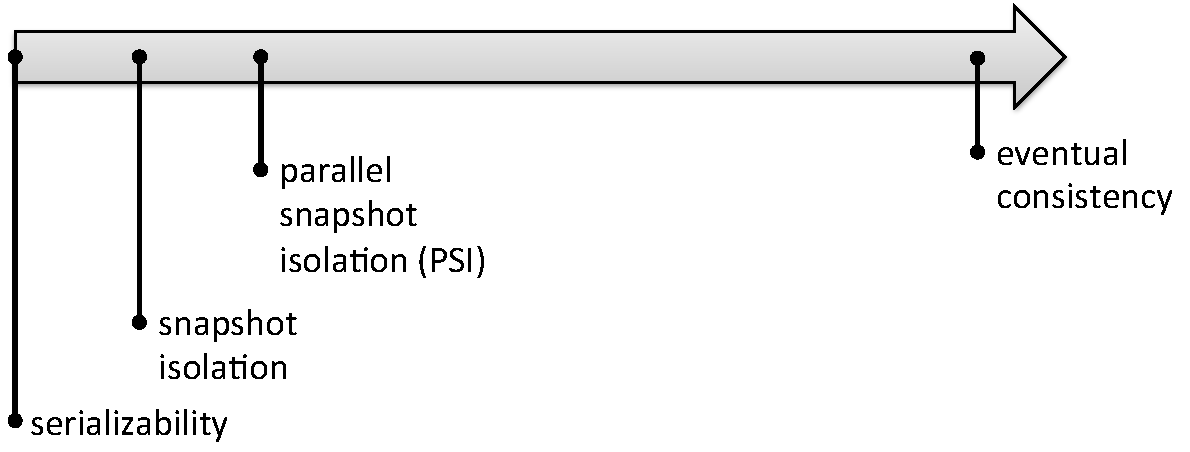
\includegraphics[width=0.5\textwidth]{figs/consistency}
\caption{Transactional Storage for geo-replicated systems from \protect\cite{Sovran:2011}}
\end{figure}

\subsection{Dependability}
	\subsubsection{Replication} % Enhance reliability and improve performance. Faul-Tolerance and Locality respectively.
	The main concerns regarding replication are at the storage layer, and there are several possible scenarios, which require each a different approach (e.g single or multi master) In the multi-master scaling is fundamental, having advantages as well as trade-offs. A good extra property to support large distributed implementations are transactions, therefore making application programming simpler without having to care about concurrency and failures, which should be dealt with at the storage layer level on each site.	
	The meaning of replication is to enhance systems reliability by having multiple copies of data at several different locations, if possible in geographically distant locations. Also, having data locality improves response times when accessing local copies of data so benefits the overall system performance implementation. There are several points to note in the following then:

\begin{itemize}
	\item{Scalability:}
	Replication is, among other things, a technique for scaling. Copying data over several locations can improve access times to local clients. A client accessing certain information can be redirected to the closest replica node available in the network of data centers. That reduces latency overhead and delays locally, although it poses a problem on the network communications required to update all other replicas once an update occurs.

	\item{Ensuring Availability and Fault-Tolerance:}
	If a replica fails there is another one which can take respond to the request and therefore avoid a single point of failure in the storage system. That creates a more robust and resilient infrastructure overall.

	\item{Load Balancing:}
	There are several strategies for that, but the most usual is having replicas located in a nearby or same data center in order to provide distribution of the incoming number of requests to the system. That approach ensures high-load peaks of requests do not overflow the systems, which is important to keep the system performing well and avoiding to slow down the processing of requests in response to clients.
\end{itemize}
	
	%\subsubsection{Availability} TODO
		
	%\subsubsection{Scalability} TODO
	
		
	%\subsubsection{Fault-Tolerance and redundancy} TODO


  %%%%%%%%%%%%%%%%%%%%%%%%%%%%%%%%%%%%%%%%%%%%%%%%%%%%%%%%%%%%%%%%%%%%%%%%%%%%%
  %
%%%%%                        LIST OF DATA STORES SECTION

%\section{Transactional support for NoSQL data stores}
\section{Typical distributed data stores in use} % list of products and their description
A full list of the types of data stores described is presented in the following sections.

\subsection{Key-Value Stores}

	\subsubsection{Voldemort}	
	Open-source follow up of Dynamo, Voldemort~\cite{Sumbaly:2012} is being used for instance at LinkedIn for providing high-scalability. The system is built for efficient but simple queries, so there is no need or support for joins (implemented at the application level). Constraints on foreign keys are also unsupported and not possible. Obviously, no triggers or views can be set up as in traditional relational database systems. These are the trade-offs that allow the system to have better performance in terms of queries, distribution of data storage, separation of concerns between logic and data model. This is as we say, in contrast to RDBMs more practical and efficient for distributed systems with need for simple APIs and object oriented paradigms in applications.
	
	One interesting aspect of Voldemort is the concept of \emph{stores}, which are namespaces of key-value pairs stored with unique key and each of them associate to only one value. Values can be still lists, maps or scalars. In one thing it resembles Amazon Dymano, as it is highly available during write operations, can tolerate concurrency during updates and causality of versions is implemented though vector clocks.

	\subsubsection{Dynamo}
	Amazon designed Dynamo, which can also use an eventual approach but in their implementation they focused more in another type of algorithms for providing direct routing with zero hops to the destination unlike Chord~\cite{Stoica:2001}. It provides a tunable R+W \textgreater N consistency model. The application programmer using Dynamo specifies the amount of replicas that one needs up to date on a read (R) or write (W). As long as R+W is greater than N, the total number of replicas, it should provide consistency to the user (assuming correctly merged writes). That means for a typical replication factor of N=3, the programmer can specify highly available writes and slower but consistent reads (3+1\textgreater3), a more balanced approach (2+2>3), or assuming a read-heavy workload (1+3\textgreater3). Increasing N increases the replication factor, meaning better durability. Choosing \text{R+W} less or equal to N allows for eventual consistency. Although one can argue Dynamo fails to fulfil the needs of datacenters based applications.
	Most services only store and retrieve data by primary key so complex querying is not required. Consistent hashing is used for partitioning and replication. Consistency is achieved through versions of objects. Being a decentralized system, nodes can be added or removed without any extra overhead. Usually that sort of system is best for applications that need a data store that tolerates writes and there are no concurrent writes failures.
	Replication is used per node, so a coordinator node is called one upon data falls within its on range and therefore assigns copies of the source data to as many other hosts as specified by N itself.


\subsection{Document Stores}
	\subsubsection{MongoDB}
	MongoDB is one of the most popular document stores. It is schema-free and supports Map-Reduce operations too. MongoDb as well, provides indexes on collections. The consistency model is eventual and uses asynchronous replication for that. Regarding atomicity, provides atomic updates on fields by tracking changes on those and updating the whole document only if that is a known-value.
	
	\subsubsection{CouchDB}
	CouchDB on the other hand uses MVCC for atomicity on documents. Consistency is not guaranteed, each client might be having a different view of the database itself. There is no replication between replica nodes, so therefore a MVCC system to control version conflicts. It is up to the application level to handle the notifications from CouchDB for updates seen since last fetch operation.
	

\subsection{Column-Stores}
	\subsubsection{HBase}
	In previously devised systems at Google, BigTable~\cite{Chang:2006} for example mainly aims to be a highly available and scalable key-value store without compromising performance. It is then with built for lexicographically sorted data and each family has the same types. It also uses several other technologies, Chubby as a locking service, Google File Systems to store logs and data files, and SSTables for BigTable data (also implemented in HBase). In Figure~\ref{hbase-architecture} we can see an architecture design of the system developed at Google and compare it to Hbase. 

%insert figure -- %Need to explain what is metadata and put small graph maybe of BigTable?%

\begin{figure}[h]
\centering
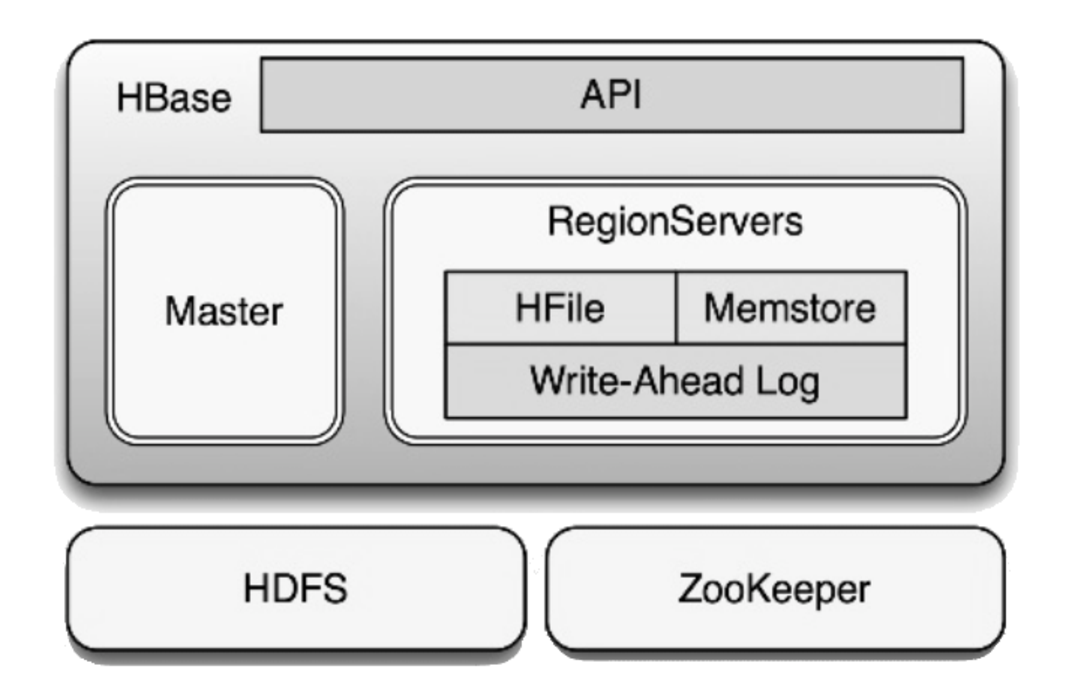
\includegraphics[width=0.5\textwidth]{figs/hbase-main-architecture}
\caption{The main HBase architecture from \protect\cite{SlidesLars}}
\label{hbase-architecture}
\end{figure}

Hbase is an open-source distributed, versioned, column-store designed after BigTable~\cite{Chang:2006}, which is also a distributed, persistent and multi-dimensional sorted map. HBase uses Zookeeper~\cite{Hunt:2010} to provide high availability and it is written in Java to managed large amounts of sparse data. The cloud data store is nowadays being used as the messaging layer at companies such as Facebook~\cite{FacebookHBase}. It has good write latency but some durability concerns (as it does not commit updates directly to disk) and not so good results in the case of reads as seen in~\cite{YCSB:2010}. The underlying file system is HDFS, analogous to GFS from Google with BigTable. In master to master replicated scenarios there are only eventual guarantees to the consistency of data, although data integrity is somehow ensured with a minimum provided set of replicas in HDFS memory of 3, claimed to be enough for the purpose.

Although that works well in most cases, more complex applications which require stronger consistency guarantees can be difficult to manage with BigTable so due to those constraints, Google developed later on in 2012 an evolution of BigTable that provided external consistency with atomic clocks and so on, Spanner~\cite{Corbett:2012}. That can make applications still benefit from high-availability while ensuring synchrony among distant replicas and more importantly, atomic schema changes. Data locality is also an important feature so partitioning of data across multiple sites is used on both BigTable and Spanner, specifically in the later to control read latency. Regarding write latency, Spanner supports that type of control by knowing how far are replicas from each other or in other words, very similarly to what had been already proposed as part of other existing middleware frameworks for HBase such as VFC$^{3}$~\cite{Vfc3:2012}.  

Performance in HBase improves as the number of servers increases due to more memory available~\cite{Carstoiu:2010}, but regardless of that fact, it is not trivial to scale always further by following the later approach. Therefore, having ways of providing different levels of consistency to users regarding data in cloud environments translates into substantial traffic savings and therefore associated costs to potential service providers or even customers, which is a very relevant matter as seen in~\cite{chihoub:2013} for consistency-cost efficiency. It is then always good to constantly be evaluating how selective replication (with a QoD in this case) can support that statement in distributed deployments with HBase.

Inside the same data center strong consistency is provided which means one can read its writes independently of what replica node is reading from. Although and as pointed out in several technical reports from Facebook~\cite{Aiyer:2012}, there is still work to do in the area of cross data center replication, which is the main aim here in the thesis work here presented and which we explain in the next chapters of the document. In master to master replicated scenarios eventual guarantees to the consistency of data are provided in HBase through mechanims based on a custom protocol with RPC calls. Therefore replicas can contain stale data in the order of seconds to minutes until the full set of updates is received.

\subsubsection{Spanner}

There has also been some recent research that addresses these shortcomings in geo-replicated data center scenarios like~\cite{Corbett:2012}. HBase does not use that Paxos either for synchronization of replicas. On the other hand, the performance of the data store for random writes and replication between remote sites is very fast and provides advantages in that area. Spanner does use Paxos for strong guarantees of replicas and that seems to work well enough, although is not really implemented with HBase it is possible to take that approach. Therefore one need to trade data availability for consistency between replicas in the presence of partitions. That is achieved through asynchronous communications rather than serializability, in order to minimize the cost of latency in wide-area scenarios with clusters running Hadoop as the storage layer of Hbase. Hadoop is good for many reasons, and frees the higher layer from other tasks and one can even implement transactions if desired on top of it.

\subsubsection{PNUTS}

On the other hand, systems as PNUTS~\cite{Cooper:2008}, yet another cloud database systems a.k.a NoSQL, Yahoo introduced a novel approach for consistency on per-record basis. Therefore being able to provided low latency during heavy replication operations for large web scale applications. They, as in our work provide a finer grain guarantees for certain data, so in other words, new updates are not always seem right away by the clients (which is the case anyway in HBase), but only if strictly necessary. Keeping that in mind, that is not always appropriate to keep the application available and performing both at once. They realize that eventual consistency is not enough in the case of social and sharing networks, as stale replicas can result in undesired cases of users having the opportunity to see or use data they were not supposed to access or so, and therefore a privacy issue as well as data consistency concerns on end users. Also, the main trade-off with PNUTS is the limited or not support for transactions.

\subsubsection{Megastore}
MegaStore is also an invention developed at Google. The main idea is to provide ACID properties across geo-located data centers with scattered data-sets and a Paxos scheme for replication. With inter data center replication Megastore can achieve fault tolerance while still providing strong consistency properties. It also scales, by partitioning data-sets into entity \emph{groups} Multi-site operations result in poor performance with Megastore, that is its main drawback. The model and language is different from those data stores such as BigTable~\cite{Chang:2006} but also from Relational Database Management Systems~\cite{RDBMS}.

\subsubsection{Azure}
There are other look alike systems such as Azure~\cite{Calder:2011} from Microsoft, which provides strong consistency on the other hand. This system tries to give priority to consistency even in the event of partitions in the network. Durability is ensured with two or more copies of the data. The systems is scalable and provides a global name-space.

Regarding its architecture, Storage Stamps are used to expand out global data center capacity. The Geo-Location service does the balancing and fail-over across different stamps across different data centers. Within a Storage Stamp, there is a Stream Layer which is append-only distributed file system which replicates data across domains. Replica recovery is possible. The Partition Layer understand what is a data structure is (blobs, queues..) and it is possible to manage the consistency of the items in the Stream Layer (persistence). Basically, the partition layer sends asynchronously the items for geo-replication. There is also a commit log similarly to the WAL in HBase, which is useful for recovery in case it is necessary.

\subsubsection{Cassandra}
Cassandra is a well known key value store system developed at Facebook for scaling of their back-end storage architecture while achieving high performance and wide applicability~\cite{Lakshman:2010}. Replication is support across multiple data centres, providing quite low latency for reads and specially writes. The key point of Cassandra is its ability to define several types of consistency, which can be configured by the user before runtime. Cassandra works similarly to HBase, using a write ahead log for durability and a Memtable to store volatile data. Atomicity is ensure at the row-level, which is none or nothing. As we we will see later in our implementation of HBase QoD, Cassandra uses a tunable data consistency model which also works for distributed environments. 

\paragraph{Scalability:}
To scale Cassandra follows a similar approach to Chord~\cite{Stoica:2001}, where the load is partitioned among the neighboring nodes to avoid the load goes on some of the existing nodes only.

\paragraph{Fault-Tolerance:}
Cassandra uses replication Quorums for ensuring data is fault tolerant. In the replication model, either all nodes respond for the write to be successful or none of them does. Read-repair occurs when obsolete data must be updated in a per request basis. That is data that will need to be up to date for an eventual "Insert", "Update" or similar operation on the database.

% Quorum -> replication factor
% 4 -> duplicate in every row
% 3-> must respond for write to be successful
%
%All -> respond from all the nodes managing information for write to be successful.

%Fault-Tolerance:
%If am writing some data in the node, 

%Read-repair ensures that obsolete data is updated in a request basis. That data will be up to date. Select, Insert, ...
\subsection{Typical distributed and replicated deployments}\label{distributed-architecture}
There is extensive work in this area of geo-replicated data stores. For instance, in proposals of systems such as D-Tunes~\cite{PN:2013} there is a clear relationship between having a self-tuning and adaptive data model that allows adjusting geo-distributed data store needs automatically, depending of a set of previously gathered statistics, to meet strict application SLAs while still achieving optimal data store performance for all, consistency, latency and high-availability.

There is an evident need for having tailored replication mechanisms that target applications that require custom levels of consistency, that has been described among others in~\cite{Kraska:2009}, where for instance a buffer is used to keep lists of pending updates for that purpose. It is also worth to mention what other techniques have or are being used for a similar purpose, such as for instance Snapshot Isolation or ALPS properties in systems like COPS~\cite{Lloyd:2011} which present novel ideas on the subject regarding consistency. Or in the well-known \emph{conit consistency model} from Duke University \cite{Duke:2001}, a system built with these same premises is also presented, but focused on generality rather than practicality. The thesis work refers more specifically to the later, as it is more rewarding to users that need to integrate a fully functional system with a replication framework that optimizes Geo-Replication. Actually there is an opened issue reported on the HBase community~\cite{JIRA-1}. In distributed clusters, Facebook is also using HBase to manage the messaging of the platform across data centers. That is in despite of Cassandra~\cite{FacebookHBase}, previously devised internally at their own company. That may be well be because of the simplicity of the consistency model as well as the ability of HBase to handle both a short set of volatile data and an ever-growing data set that rarely gets accessed more than once. In practice, their architecture comprises a Key for each element is the userID as RowKey, word as Colum and messageID as Version and finally the value like offset of word in message (Data is sorted as: userId, word, messageID). That implicitly means that searching for the top messageIDs of an specific user and word is easily supported, and therefore queries can run faster in the backend.

%In distributed clusters Facebook is currently using HBase to manage the messaging information across data centers. That is because of the simplicity of its consistency model, as well as the ability of HBase to handle both a short set of volatile data and ever-growing data, that rarely gets accessed more than once. More specifically, in their architecture reports, a Key for each element is the userID as RowKey, word as Colum and messageID as Version and finally the value like offset of word in message (Data is sorted as: \emph{userId, word, messageID}). That implicitly means that searching for the top messageIDs of a specific user and word is easily supported, and therefore queries run faster in the backend.


%So, for filtering purposes, with our new proposal and implementation, that could directly enable administrators of the clusters to create quality-of-data policies that can analyze fetched data  isrt by inspecting some given bounds or semantics, and then receiving them on the master server at the other end of the replication chain if a match occurs. At first, we will be enhancing the eventual consistency model for inter-site replication in HBase by using an adaptive consistency model based on Service Level Objectives agreed or defined. The idea can be somehow similar to the "pluggable replication framework" proposed within the HBase community [ref here], so our work is two-fold purpose. First contributing to the open source community of HBase but also extending it with some extra capabilities, for that later we will implement batching of updates within our QoD framework.


\subsubsection{Google Cloud Data Store}
Google Cloud Datastore has been recently released. That is a system that is subject to exploration yet so we will cover limited aspects of it here. The API enables users to use a a fully managed, schema-less database on the cloud for storing their non-relational data.

There are a few key points such as ACID properties of transactions or High-Availability, Google outlines in their main website~\cite{GoogleCloudDataStore}. More interestingly also provides a differentiated approach to consistency. Strong consistency for certain reads and eventual for the rest of the queries. The reason for giving stronger consistency to some queries over others with just eventual is allowing the database performance to optimize on the overhead of strong consistency between groups of non-related items. To the contrary, with related entities, such as [Person:GreatGrandpa, Person: Grandpa, Person:Dad, Person:Me] it is by default possible with ancestor queries to use stronger consistency. Transactions are also implemented between entity groups to ensure data consistency in cases of concurrent updates to the database. As they note, to conserve memory a query should, whenever possible, specify a limit on the number of results returned, that is why.

To us, this concept is also interesting as it seems to make use of the right tools depending of what type of data is being used in order to maintain as much consistency as possible at a low-cost.

\subsubsection{MapReduce Framework}
In the MapReduce framework~\cite{Dean:04}, replication is used for tolerating failures and also performance wise. The framework was first introduced by Google and used and underlying file system called Google File System (GFS)~\cite{Ghemawat:03}. Here files are organized into chunks which are replicated to other nodes for fault-tolerance. The processing of map tasks involves the task scheduler and it is performed leveraging data locality information kept in the metadata storage, for instance first asking for the chunks required to complete tasks at the current node, in another in the same location (data center) or else outside in a completely different location, in that order of priority. That also ensures fault-tolerance and improves task average time completion by using more nodes with the relevant data available in order to speed up the process by contributing to the overall computation in parallel with the rest.



  %
 %%%
%%%%%                           THE END
  %
  %%%%%%%%%%%%%%%%%%%%%%%%%%%%%%%%%%%%%%%%%%%%%%%%%%%%%%%%%%%%%%%%%%%%%%%%%%%%%
